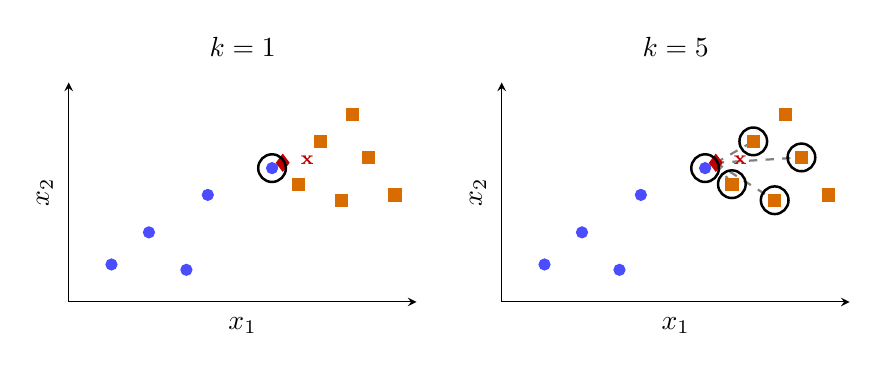
\begin{tikzpicture}
    \begin{axis}[
        width=6cm,
        height=4.5cm,
        xmin=0.5, xmax=7,
        ymin=0.5, ymax=4.6,
        axis lines=left,
        axis equal image,
        xlabel={$x_1$},
        ylabel={$x_2$},
        xlabel near ticks,
        ylabel near ticks,
        xtick=\empty,
        ytick=\empty,
        title={\(k=1\)},
        clip=false
    ]
        \addplot[only marks, mark=*, mark size=2pt, blue!70]
        coordinates {
            (1.3,1.2) (2.0,1.8) (2.7,1.1) (3.1,2.5) (4.3,3.0)
        };

        \addplot[only marks, mark=square*, mark size=2.2pt, orange!85!black]
        coordinates {
            (4.8,2.7) (5.2,3.5) (5.6,2.4)
            (6.1,3.2) (6.6,2.5) (5.8,4.0)
        };

        \addplot[only marks, mark=diamond*, mark size=3pt, red!75!black]
        coordinates {(4.5,3.1)};

        \addplot[only marks, mark=o, mark size=5pt, black, line width=0.9pt]
        coordinates {(4.3,3.0)};

        \draw[dashed, thick, gray]
            (axis cs:4.5,3.1) -- (axis cs:4.3,3.0);

        \node[font=\scriptsize, red!75!black, anchor=west]
            at (axis cs:4.65,3.15) {\(\mathbf{x}\)};
    \end{axis}
    \qquad
    \begin{axis}[
        xshift=5.5cm,
        width=6cm,
        height=4.5cm,
        xmin=0.5, xmax=7,
        ymin=0.5, ymax=4.6,
        axis lines=left,
        axis equal image,
        xlabel={$x_1$},
        ylabel={$x_2$},
        xlabel near ticks,
        ylabel near ticks,
        xtick=\empty,
        ytick=\empty,
        title={\(k=5\)},
        clip=false
    ]
        \addplot[only marks, mark=*, mark size=2pt, blue!70]
        coordinates {
            (1.3,1.2) (2.0,1.8) (2.7,1.1) (3.1,2.5) (4.3,3.0)
        };

        \addplot[only marks, mark=square*, mark size=2.2pt, orange!85!black]
        coordinates {
            (4.8,2.7) (5.2,3.5) (5.6,2.4)
            (6.1,3.2) (6.6,2.5) (5.8,4.0)
        };

        \addplot[only marks, mark=diamond*, mark size=3pt, red!75!black]
        coordinates {(4.5,3.1)};

        \addplot[only marks, mark=o, mark size=5pt, black, line width=0.9pt]
        coordinates {
            (4.3,3.0) (4.8,2.7) (5.2,3.5) (5.6,2.4) (6.1,3.2)
        };

        \draw[dashed, thick, gray]
            (axis cs:4.5,3.1) -- (axis cs:4.3,3.0);

        \draw[dashed, thick, gray]
            (axis cs:4.5,3.1) -- (axis cs:4.8,2.7);

        \draw[dashed, thick, gray]
            (axis cs:4.5,3.1) -- (axis cs:5.2,3.5);

        \draw[dashed, thick, gray]
            (axis cs:4.5,3.1) -- (axis cs:5.6,2.4);

        \draw[dashed, thick, gray]
            (axis cs:4.5,3.1) -- (axis cs:6.1,3.2);

        \node[font=\scriptsize, red!75!black, anchor=west]
            at (axis cs:4.65,3.15) {\(\mathbf{x}\)};
    \end{axis}
\end{tikzpicture}
